\documentclass{article}
\usepackage[utf8]{inputenc}
\usepackage{graphicx}
\usepackage{epstopdf}
\usepackage{float}
\usepackage[margin=1.25in]{geometry}
\usepackage{amsmath}
\usepackage{amssymb}
\usepackage{color} 
\usepackage{fancyvrb} 
\newcommand{\Vg}{{$V_{G}$}}
\newcommand{\Vsb}{{$V_{SB}$}}
\newcommand{\Vgb}{{$V_{GB}$}}
\newcommand{\Vds}{{$V_{DS}$}}
\newcommand{\Vs}{{$V_{S}$}}
\newcommand{\Vbs}{{$V_{BS}$}}
\newcommand{\Va}{{$V_{A}$}}
\newcommand{\Vd}{{$V_{D}$}}
\newcommand{\Vdd}{{$V_{dd}$}}
\newcommand{\If}{{$I_{F}$}}
\newcommand{\Ir}{{$I_{R}$}}
\newcommand{\Vt}{{$V_{T0}$}}
\newcommand{\Ut}{{$U_T$}}
\newcommand{\Is}{{$I_{s}$}}
\newcommand{\Isat}{{$I_{sat}$}}
\newcommand{\gm}{{$g_{m}$}}
\newcommand{\gmro}{{$g_{m}r_{o}$}}
\newcommand{\gs}{{$g_{s}$}}
\newcommand{\ro}{{$r_{o}$}}
\newcommand{\Vdssat}{{$V_{DSSat}$}}
\newcommand{\Vsdsat}{{$V_{SDSat}$}}
\newcommand{\nMOS}{{\textit{n}MOS }}
\newcommand{\pMOS}{{\textit{p}MOS }}

\title{Circuits Lab 6}
\author{Cory Dolphin and Noam Rubin}
\date{April 3, 2013}



\begin{document}

\maketitle
\section*{Experiment 1}

\begin{figure}[H]
\centering
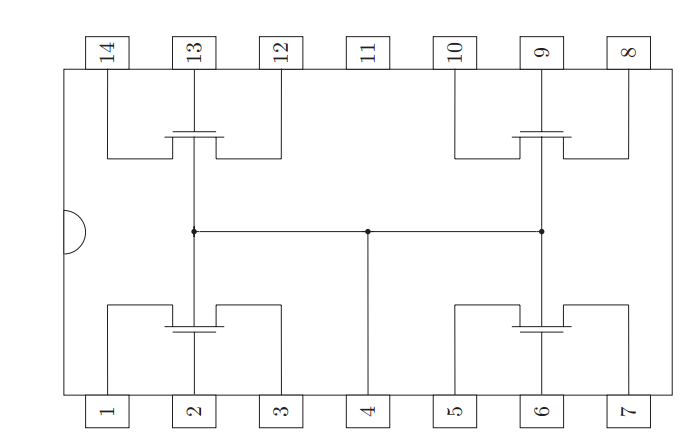
\includegraphics[width=0.65\linewidth]{../Figures/ald1106}
\caption{Picture of the ALD1106 QUAD nMOS transistor array which was used in Experiment 1 to analyze the similarities between nMOS transistors. Using a Quad array is ideal as all transistors are manufactured on the same substrate, optimizing their similarity.}
\label{fig:ald1106}
\end{figure}


In this experiment, we wanted to evaluate how well-matched four nMOS transistors on the same die are. We used the ALD1106 Quad nMOS array, as seen in figure \ref{fig:ald1106}, as all four transistors on this chip are manufactured on the same substrate, which optimizes their similarity.

\begin{figure}[H]
\centering
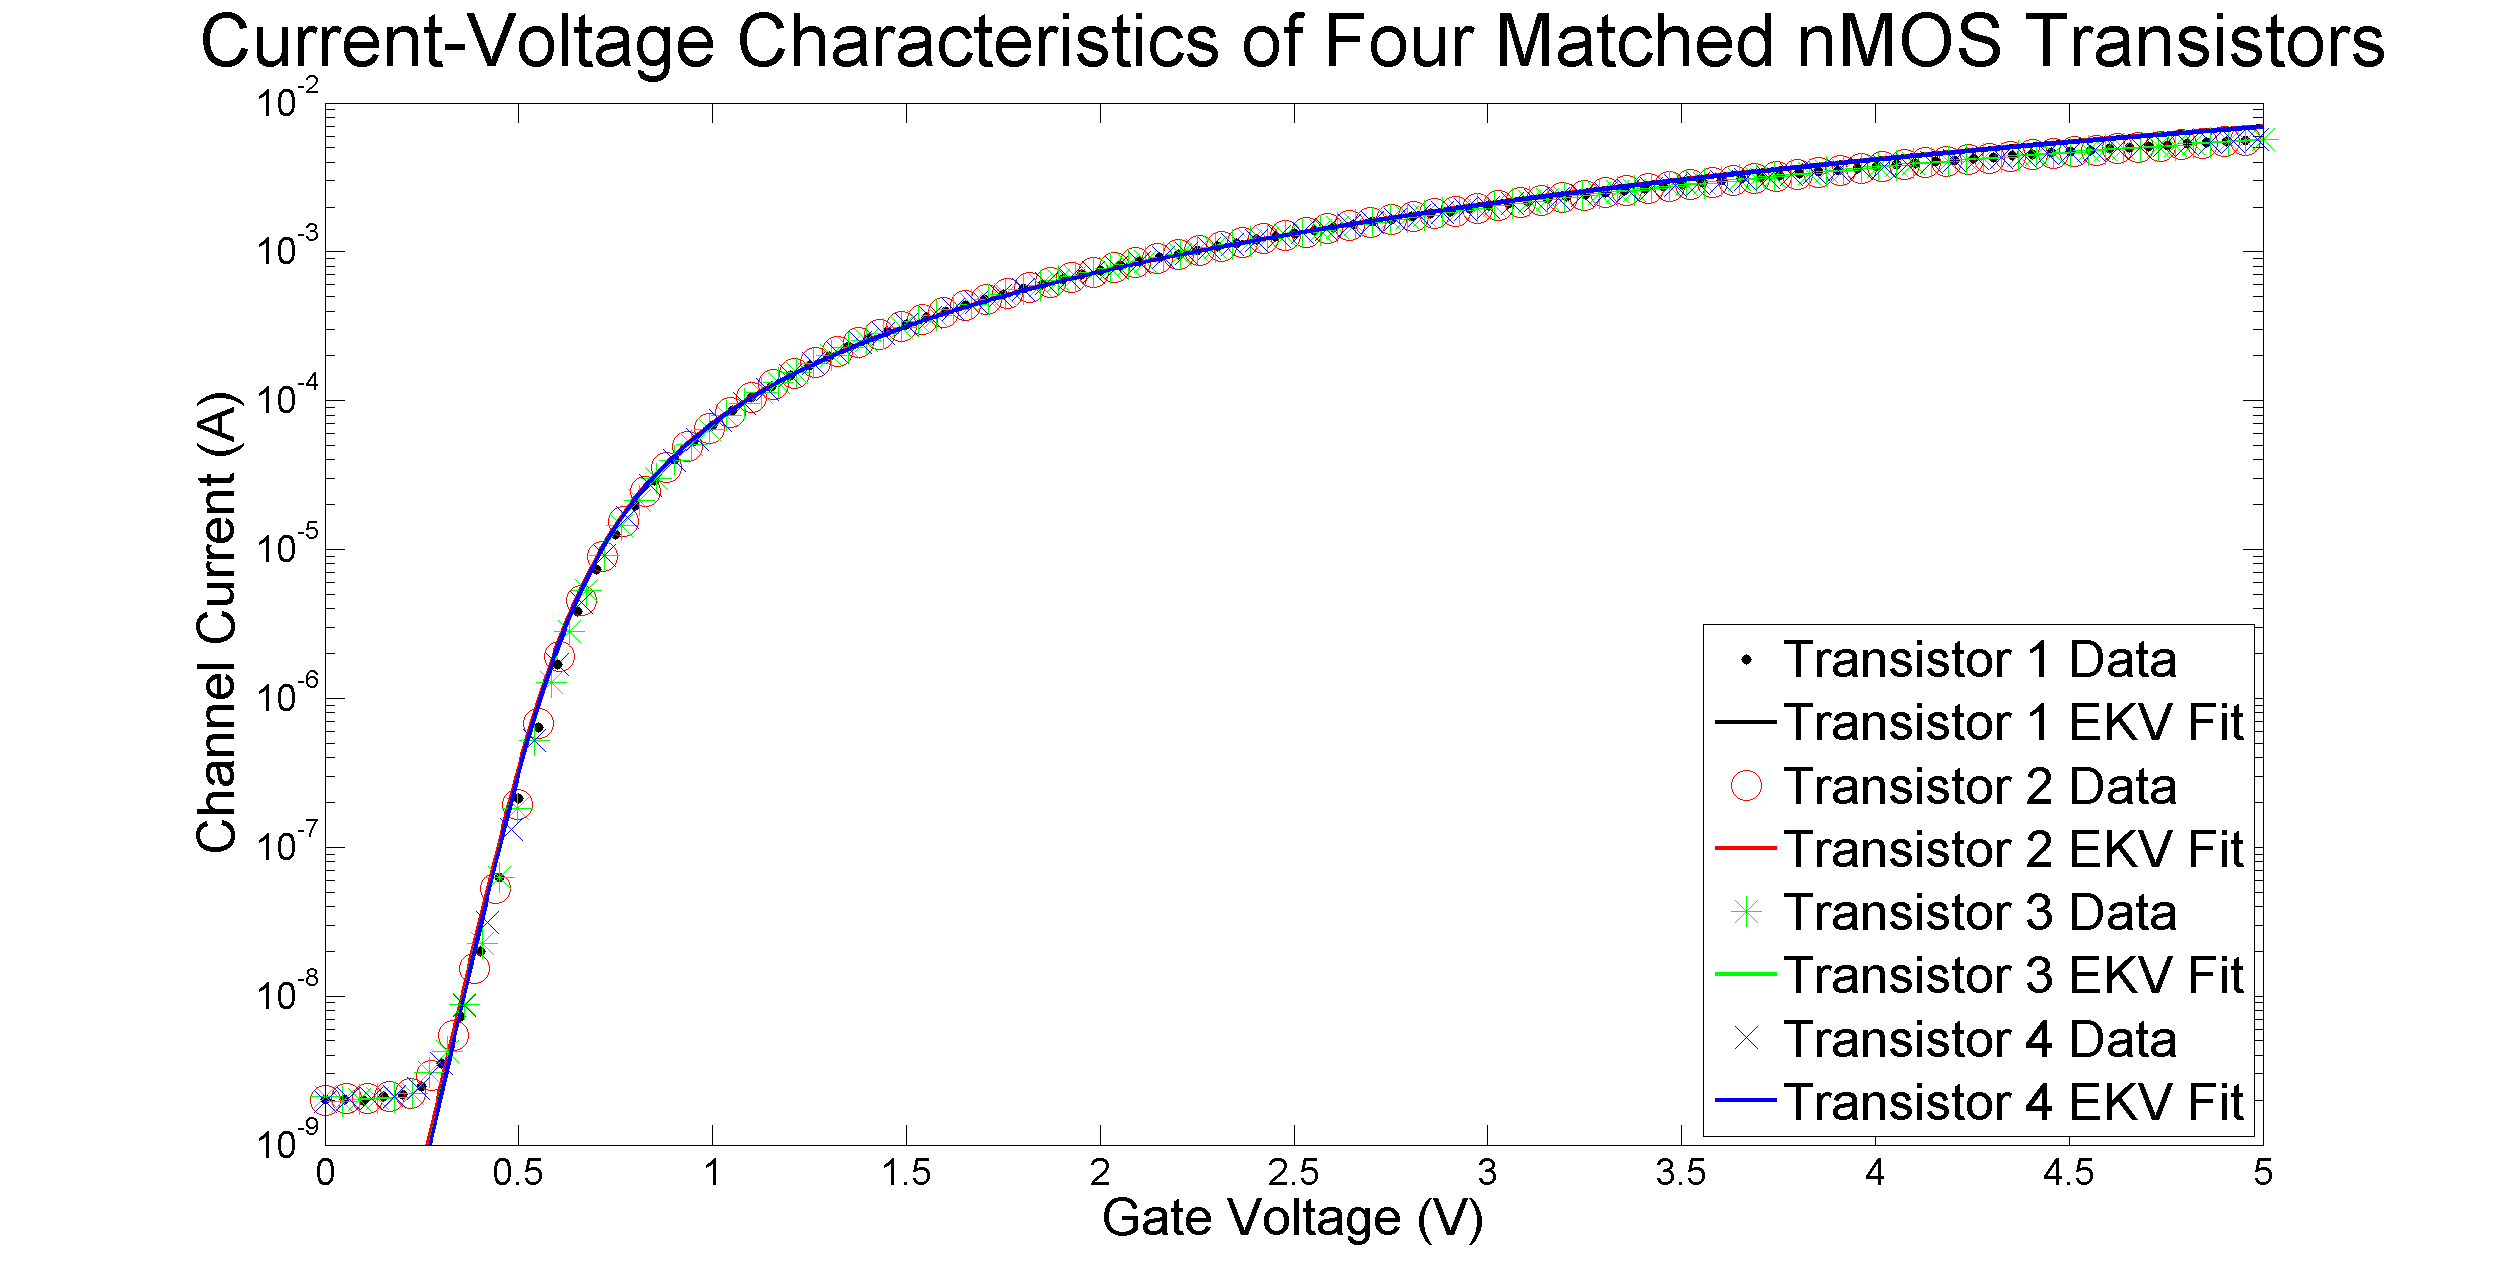
\includegraphics[width=0.65\linewidth]{../Figures/Experiment1Figure1.eps}
\caption{Picture of the ALD1106 QUAD nMOS transistor array which was used in Experiment 1 to analyze the similarities between nMOS transistors. Using a Quad array is ideal as all transistors are manufactured on the same substrate, optimizing their similarity.}
\label{fig:exp1fig1}
\end{figure}
\begin{figure}[H]
\centering
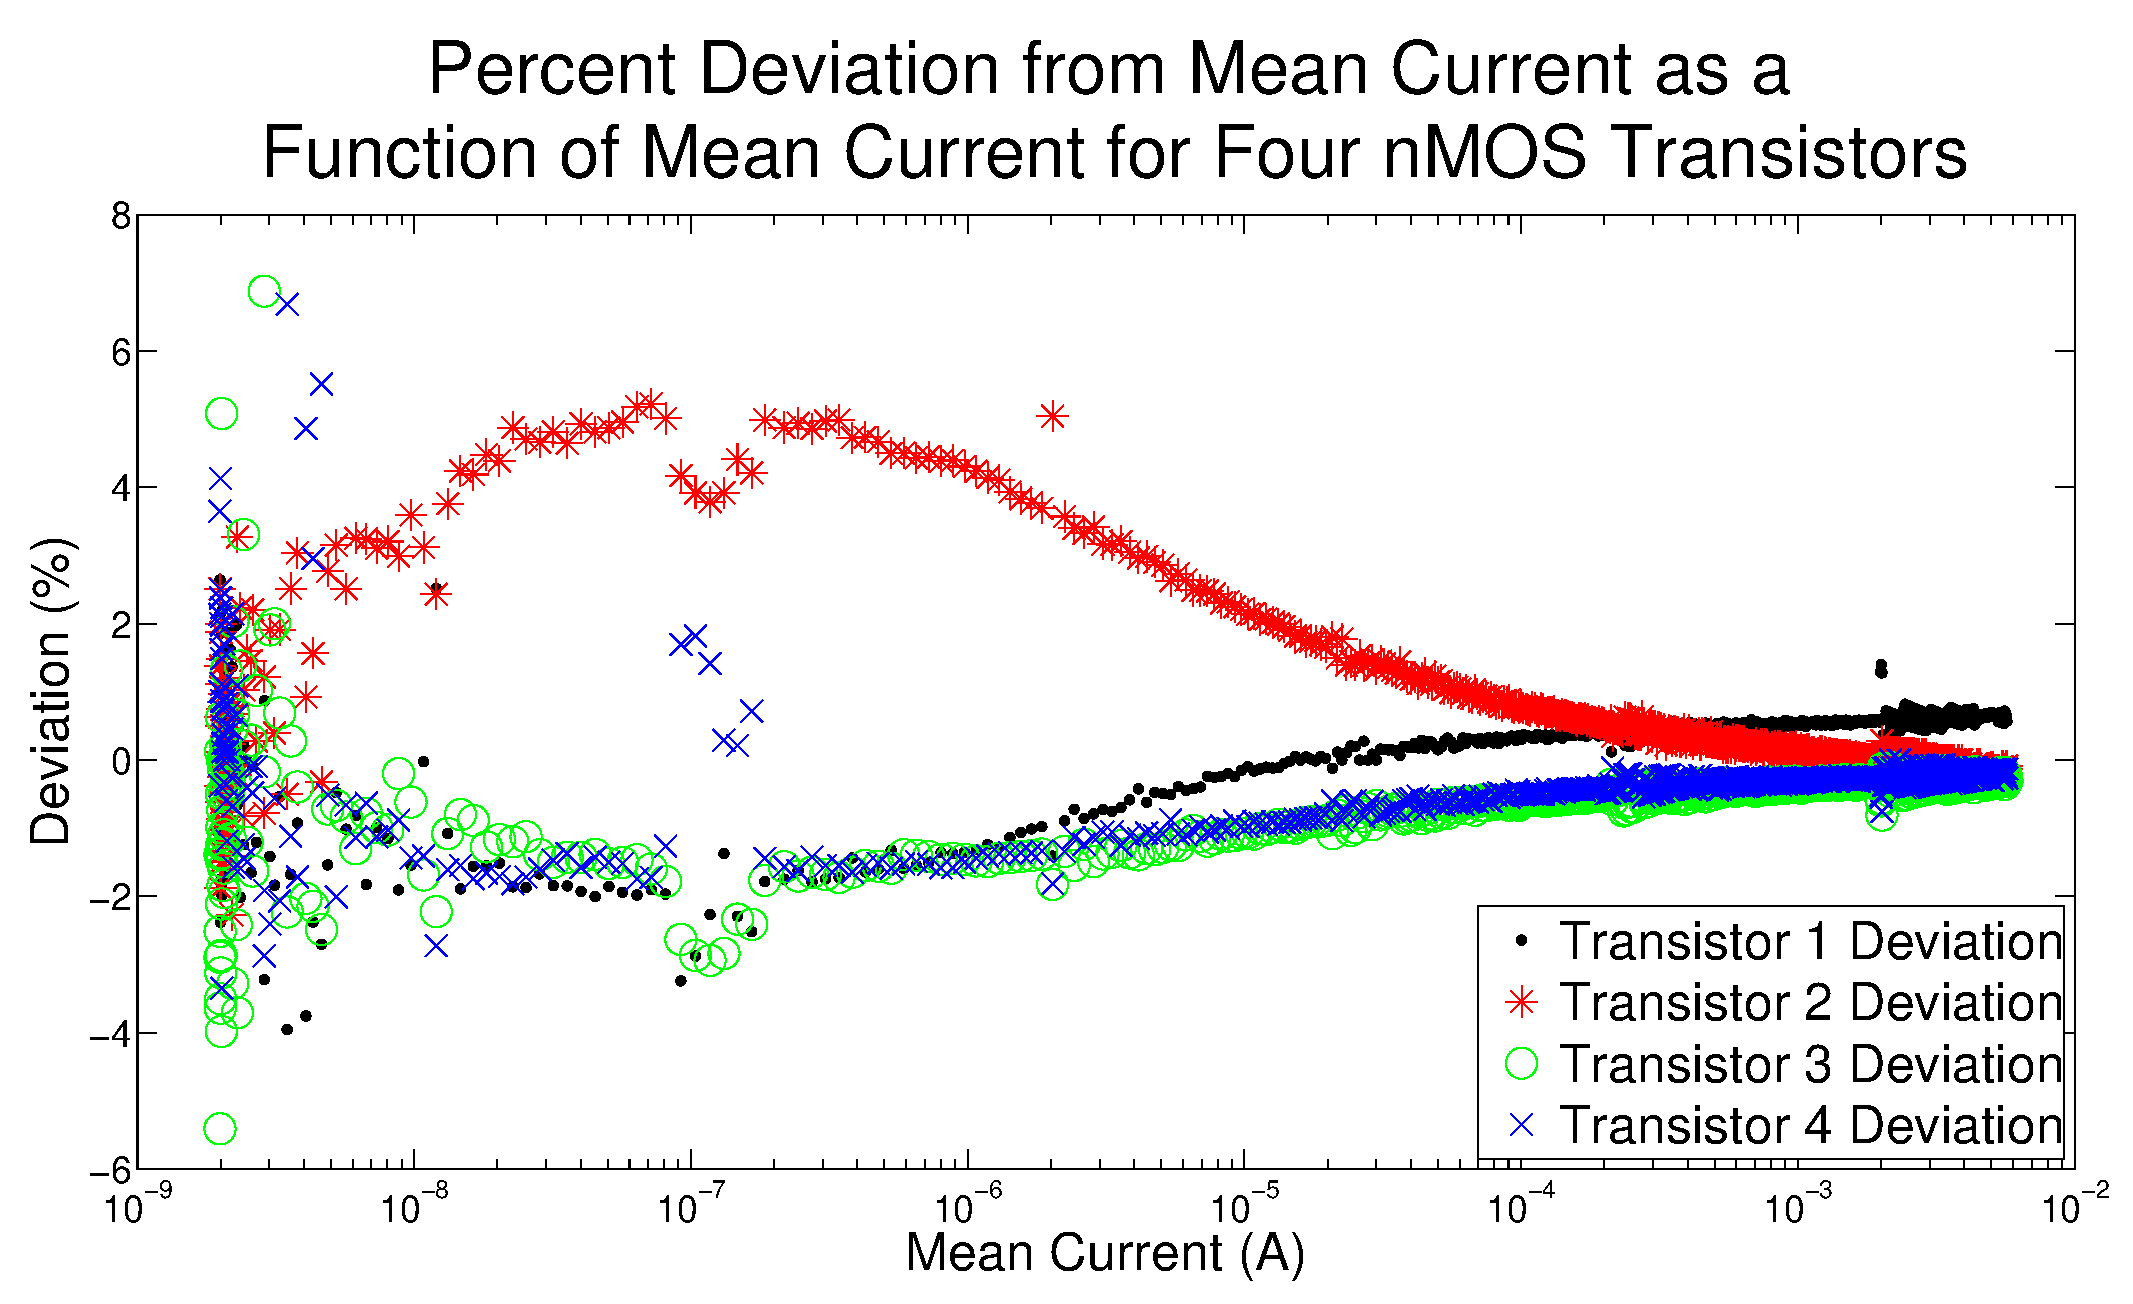
\includegraphics[width=0.65\linewidth]{../Figures/Experiment1Figure2.eps}
\caption{Picture of the ALD1106 QUAD nMOS transistor array which was used in Experiment 1 to analyze the similarities between nMOS transistors. Using a Quad array is ideal as all transistors are manufactured on the same substrate, optimizing their similarity.}
\label{fig:exp1fig2}
\end{figure}
\section*{Experiment 2}
In this experiment, we explore how series and parallel combinations of \nMOS transistors behave, 
and what affect these combinations have on the channel current, \Isat, as a function of gate voltage,
\Vg. In order to accomplish this comparison, we collected data for the channel current in both ohmic 
and saturation regions of operation for a single \nMOS transistor, two transistors in parallel, and
two transistors in series, using $V_{gb} = 10mV$ and $ V_{ds} = V_{dd}$ and respectively.

\begin{figure}[H]
\centering
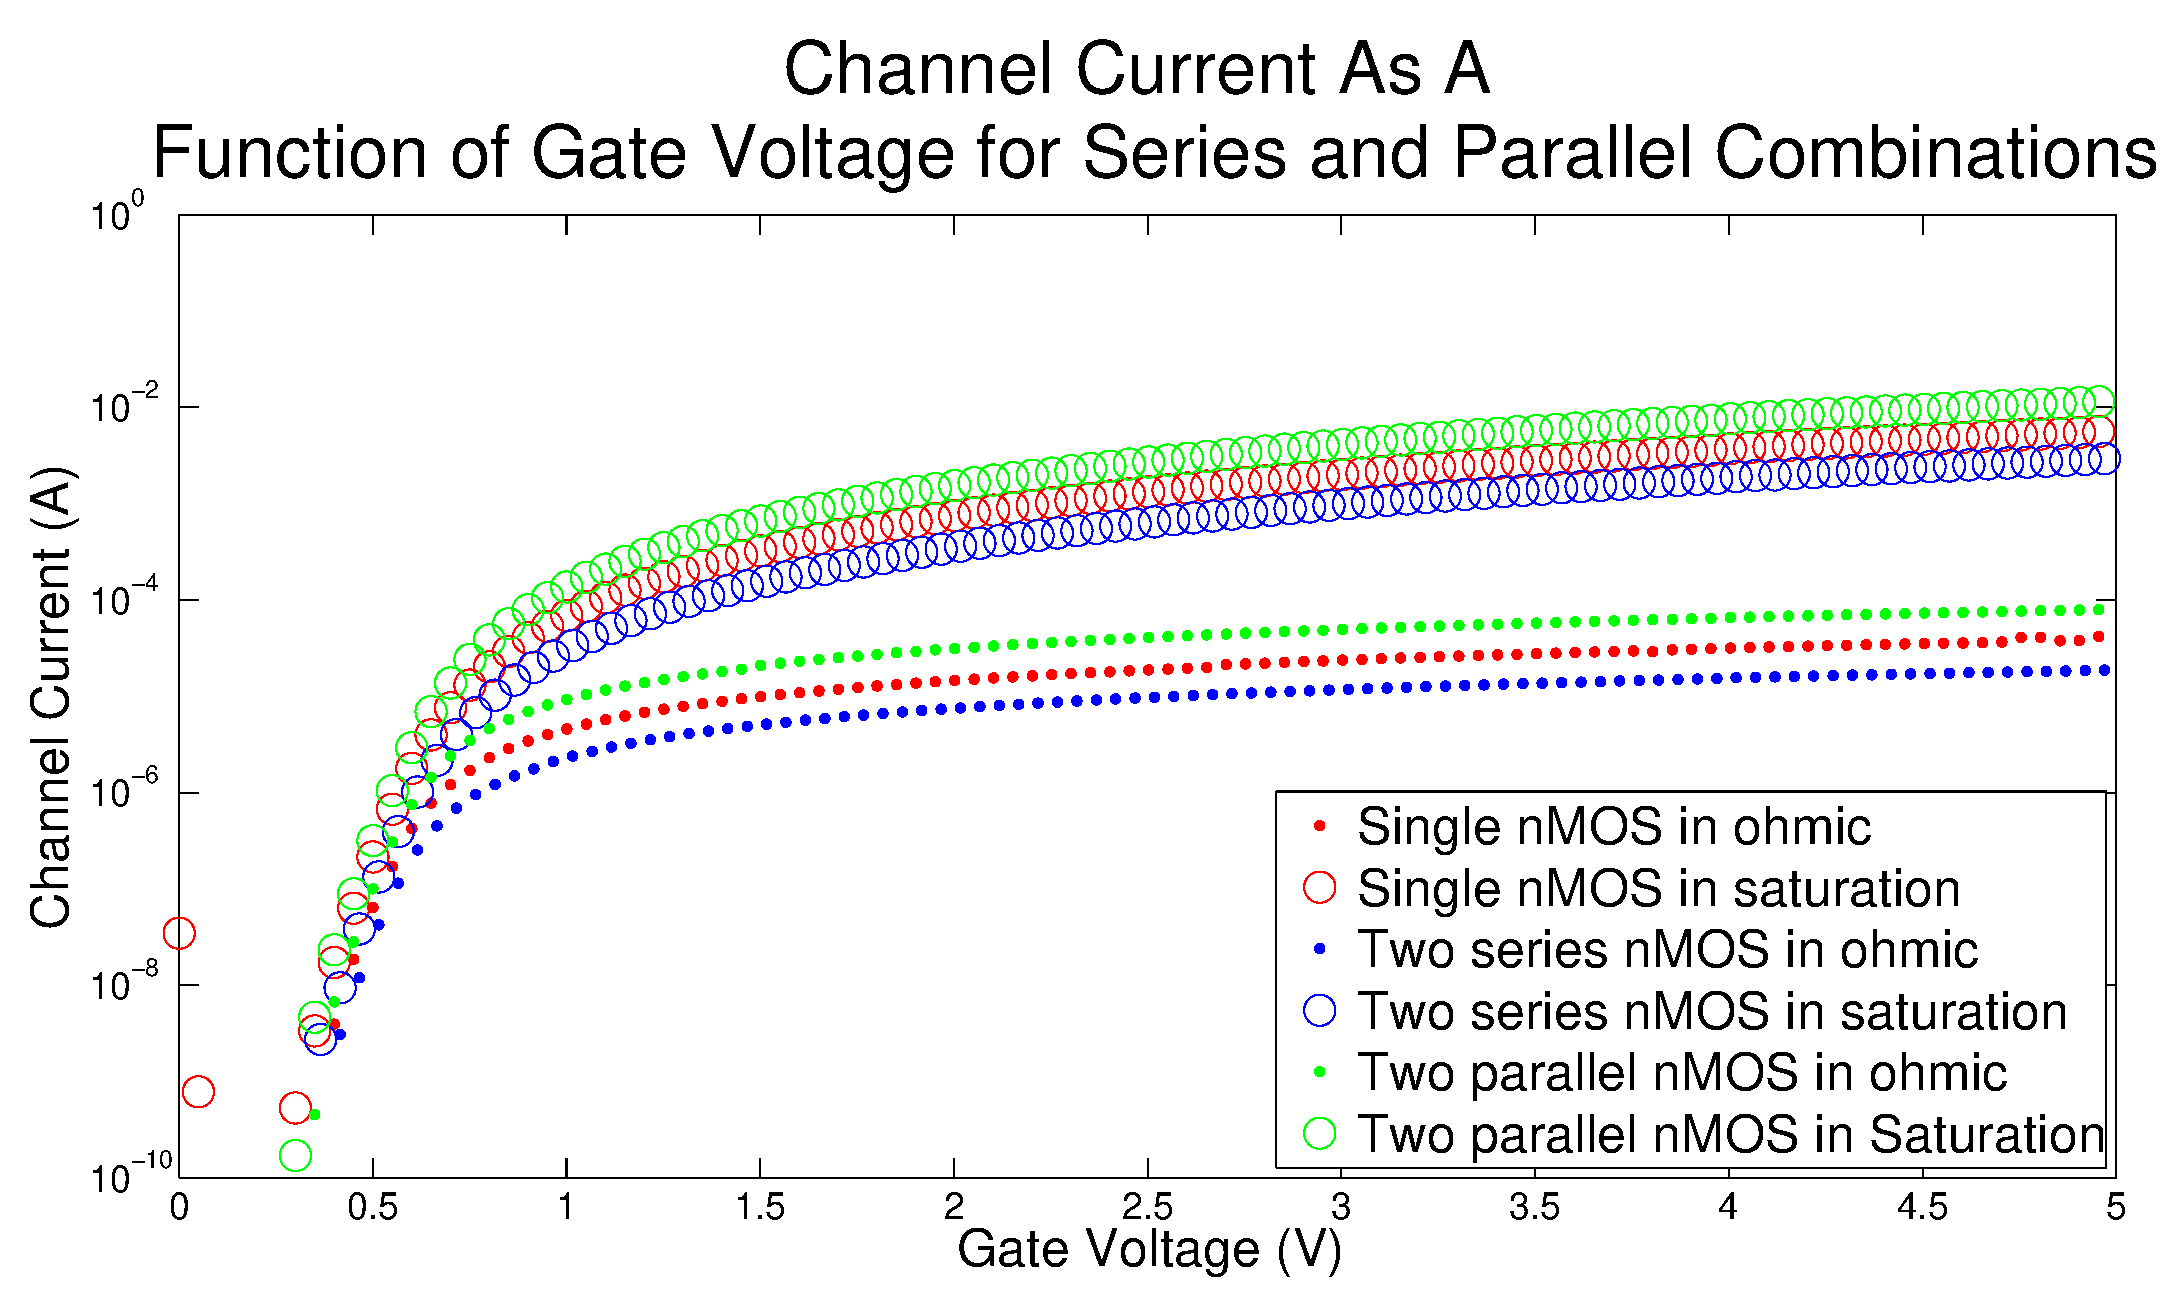
\includegraphics[width=\linewidth]{../Figures/Experiment2Currents.eps}
\caption{}
\label{fig:nmosdia}
\end{figure}
\end{document}